\documentclass[12pt]{article}

\usepackage{preamble}
\usepackage{hyperref}

\begin{document}

\textbf{EN.580.475.}

Daniel Yao

\today

\textbf{Introduction.}

Brawl Stars is a 3v3 mobile game developed by Supercell. The competitive format proceeds in two stages: the draft and the gameplay.

First, the game mode (there are six total) is revealed. Two teams, Blue and Red, each independently choose 3 of 97 brawlers to ban. These bans are then revealed. Blue chooses one brawler, Red chooses two brawlers, Blue chooses two brawlers, and then Red chooses one brawler. These brawlers are chosen without replacement so that each team has three brawlers and that these brawlers are unique. The players then play the game mode with their chosen brawlers, and the victor is decided in a best of three contest.

In the past few years, the competitive community has come to jokingly refer to the game as "Draft Stars", due to the increasing importance of the draft stage over the gameplay stage with the addition of new characters.

I address this draft stage. First, I train three models (logistic regression, random forest, and neural network) to predict the game outcome given a draft. I evaluate these three models and select the best one. I then propose a mini-max algorithm to determine the optimal draft order using this model. Finally, I address the (many) limitations of my method.

\textbf{Data collection.}

I obtained the data during the summer of 2024 through BrawlStarsAPI. There are 5514 games with 82 unique brawlers. (There were fewer brawlers in the game at the time.) Though the data are old, the analysis is new.

Since the modes and brawlers are categorical and their is no meaningful order to these categories, the data are one-hot encoded. There are 6 modes and 82 choices for six players, for a total of 
$$6 + 6(82) = 498$$
dimensions.

\textbf{Logistic regression.}

\textbf{Random forest.}

\textbf{Neural network.}

I train an neural network with two hidden layers of 256 neurons, ReLU activations, sigmoid output, and BCE loss.

\begin{center} 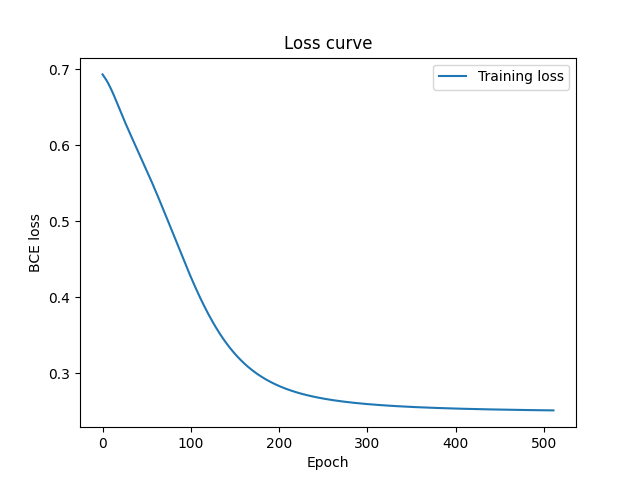
\includegraphics{"../output/nn_loss_curve.png"} \end{center}

We see that this neural network can predict the victor with better than average chance, but it grossly overfits the training data. Indeed, the training loss converges after 500 epochs, but the testing accuracy converges after only 100 epochs.

\textbf{Results.}

\textbf{Discussion.}

\textbf{Application.}

\textbf{Conclusion.}

\begin{center} 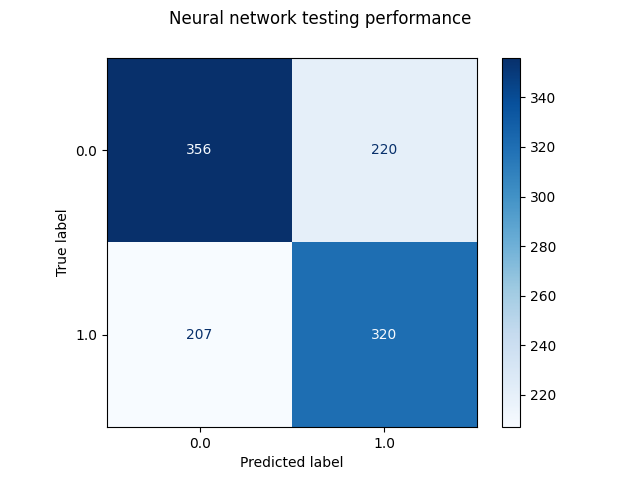
\includegraphics{"../output/nn_testing_confusion_matrix.png"} \end{center}

Nevertheless, it is impressive that 

\textbf{Code availability.}

\href{https://github.com/dyao13/580_475_FA25}{github.com/dyao13/580\_475\_FA25}

\end{document}